\documentclass[acmsmall,screen,nonacm,review]{acmart}

\usepackage{tikz}
\usetikzlibrary{graphs,graphs.standard}
\usepackage[textsize=small]{todonotes}
\newcommand{\rw}[1]{\todo[inline,color=cyan!60]{\sf RW: #1}}
\newcommand{\dan}[1]{\todo[inline,color=red!60]{\sf DS: #1}}
\newcommand{\yz}[1]{\todo[inline,color=green!60]{\sf YZ: #1}}

\newcommand{\homeq}{\equiv}
\newcommand{\iso}{\simeq}

\newcommand{\set}[1]{\{#1\}}                    % Set (as in \set{1,2,3}).
\newcommand{\setof}[2]{\{{#1}\mid{#2}\}}        % Set (as in \setof{x}{x>0}).
\newcommand{\N}{{\mathbb N}}                            % Expectation
\newcommand{\R}{{\mathbb R}}                            % Expectation
\newcommand{\Z}{{\mathbb Z}}                            % Expectation
\newcommand{\defeq}{\stackrel{\text{def}}{=}}
\newcommand{\dom}{\textsf{Dom}}
\newcommand{\arity}{\textit{ar}}



\begin{abstract}
The chase is an important tool in databases.
Among the different variations of the chase, 
 the core chase arguably has the best properties:
 it is the only variant that guarantees to compute 
 a finite solution whenever one exists, 
 and it always finds the smallest solution, called the core.
In this article, we generalize the core chase to the infinite case 
 and study its behavior when it does not terminate.
\end{abstract}

\begin{document}

\title{The Infinite Core Chase}

\maketitle

\section{Infinite Cores}

\begin{definition}
    A {\em signature} $\Sigma$ is a set of relation symbols, 
    each with an associated arity.
    A {\em $\Sigma$-structure} is a tuple $(U, I)$ where $U$ is a set, 
    called the {\em universe}, and $I$ is a function, called the {\em interpretation},
    that maps each relation symbol $R$ to a relation $I(R) \subseteq U^{\arity(R)}$. 
    We sometimes identify each relation $I(R)$ with its symbol $R$, 
    and the interpretation with the set of all relations, 
    as well as with structure itself.
    We write $R(a_1, \ldots, a_n)$ for the tuple $(a_1, \ldots, a_n) \in R$.
\end{definition}

\begin{definition}
    A {\em homomorphism} between two $\Sigma$-structures $(U, I)$, $(V, J)$
    is a function $h: U \to V$ such that for every relation $R$,
    if $I(a_1, \ldots, a_n) \in I$ then $R(h(a_1), \ldots, h(a_n)) \in J$.
    We extend a homomorphism $h$ to tuples, relations, and structures 
    in the natural way.
    In particular: 
\begin{align*}
    h(R(a_1, \ldots, a_n)) & \defeq (R(h(a_1), \ldots, h(a_n))) \\
    h(R) & \defeq \setof{h(t)}{t \in R} \\
    h(I) & \defeq \setof{h(R)}{R \in I}
\end{align*}
We call the image of $h$ the {\em homomorphism image}.
\end{definition}

\begin{definition}
    We call a homomorphism from a structure to itself an {\em endomorphism}.
\end{definition}

\begin{definition}
    Two structures $I$, $J$ are {\em homomorphically equivalent}, 
    written $I \homeq J$,
    if there are homomorphisms $h: I \to J$ and $g: J \to I$.
\end{definition}

\begin{definition}
    An {\em isomorphism} between two strucutres $I$, $J$ 
    is a function $f: I \rightarrow J$ that 
    has an {\em inverse} $f^{-1}: J \rightarrow I$
    such that $f^{-1} \circ f (I)= I$ and $f \circ f^{-1} (J) = J$.
    We say the structures are {\em isomorphic}, written $I \iso J$.
\end{definition}

\begin{definition}
    A structure $I$ is a {\em core} if every endomorphism image 
    of $I$ is isomorphic to $I$.
    A substructure $H \subseteq I$ is called a {\em core of} $I$
    if there is a homomorphism $h: I \rightarrow H$, and $H$ is a core.
\end{definition}

Note that the definition of core for infinite structures is not standard, 
 and we carefully chose our definition to ensure several desirable properties, 
 as we shall see.

\begin{lemma}\label{lem:core-iso}
    Two homomorphically equivalent cores are isomorphic.
\end{lemma}
\begin{proof}
    Let $I, J$ be the cores,
    and $h_1: I \rightarrow J$, $h_2: J \rightarrow I$ be 
    homomorphisms between them.
    Because $h_2 \circ h_1 : I \rightarrow I$ is an endomorphism, 
    and $I$ is a core, $I \iso h_2 \circ h_1(I)$.
    Call this isomorphism $i_1$, and we have $i_1 \circ h_2 \circ h_1(I) = I$.
    By definition $h_1(I) \subseteq J$, 
    so $I = i_1 \circ h_2 \circ h_1(I) \subseteq i_1 \circ h_2(J)$.
    But $i_1 \circ h_2(J) \subseteq I$,
    we must have $I = i_1 \circ h_2(J)$.
    Similarly, we can define an inverse mapping from $I$ to $J$
    as $J = i_2 \circ h_1$, where $i_2$ is an isomorphism on 
    $J$ defined similarly as $i_1$.
    Together, $i_1 \circ h_2$ and $i_2 \circ h_1$ define an isomorphism 
    between $I$ and $J$.
\end{proof}

\begin{corollary}
    Homomorphically equivalent structures have the same core up to isomorphism.
\end{corollary}
\begin{proof}
    Let $I_1, I_2$ be homomorphically equivalent structures, 
    and let $h_1: I_1 \rightarrow I_2$ and $h_2: I_2 \rightarrow I_1$
    be homomorphisms between them.
    Let $H_1, H_2$ be cores of $I_1, I_2$ respectively.
    Then there are homomorphisms $r_1: I_1 \rightarrow H_1$ 
    and $r_2: I_2 \rightarrow H_2$,
    as well as $s_1: H_1 \rightarrow I_1$
    and $s_2: H_2 \rightarrow I_2$.
    We can construct a pair of homomorphisms 
    $r_2 \circ h_1 \circ s_1: H_1 \rightarrow H_2$
    and $r_1 \circ h_2 \circ s_2: H_2 \rightarrow H_1$,
    showing $H_1$ and $H_2$ are homomorphically equivalent.
    By Lemma~\ref{lem:core-iso}, they are isomorphic.
\end{proof}
\rw{Is it possible to have 2 homomorphically equivalent structures 
 where one has a core but the other does not?}
\begin{corollary}
    The core of a structure, if it exists, is unique up to isomorphism.
\end{corollary}

\subsection{Existence of the Core}
Finite structures always have a core.
This is however not obvious for infinite structures.
Bauslaugh~\cite{DBLP:journals/dm/Bauslaugh95} considers 
 several alternative definitions of core for infinite structures,
 and claims that there exist structures that do not have a core
 under any of these definitions.
As we shall see in Section~\ref{sec:related-core}, our definition
 may not be directly comparable with Bauslaugh's definitions.
We'd like to understand if all infinite structures have a core
 under our definition.

\begin{figure}
    \centering
    \includegraphics{fig/ray.eps}
    \caption{The ray graph.}
    \Description{Ray graph.}
    \label{fig:ray-graph}
\end{figure}

\begin{figure}
    \centering
    \includegraphics{fig/spine.eps}
    \caption{The spine graph.}
    \Description{Spine graph.}
    \label{fig:spine-graph}
\end{figure}

In the finite case, a simple method to find the core is to 
 repeatedly apply homomorphisms until a fixpoint.
However, for infinite structures, there can be an infinite 
 sequence of homomorphisms.
\begin{example}
Consider the graph in Figure~\ref{fig:ray-graph}, 
 taken from an example by Bauslaugh~\cite{bauslaugh1994homomorphisms}.
An endomorphism of this graph maps each vertex $i$ to $i+1$, 
 and we can repeat this mapping ad infinitum.
\end{example}
There can even be an infinite sequence of homomorphism images, 
 where none of them is isomorphic to each other.
\begin{example}
    Consider the graph in Figure~\ref{fig:spine-graph}.
    There is a sequence of homomorphisms, such that the $i$-th
    homomorphism image maps $j'$ to $j$ for $j \leq i$, 
    and maps every other vertex to itself.
    In other words, we ``fold down'' one additional ``spike''
    for every new homomorphism in the sequence.
    None of the homomorphism images in the sequence are isomorphic to each other.
    Nevertheless, the graph has a core, namely the ray graph in Figure~\ref{fig:ray-graph}.
\end{example}

Bodirsky~\cite{DBLP:journals/lmcs/Bodirsky07} proved 
 every $\omega$-categorical structure has a substructure 
 satisfying $I$ and $N$.
% 
\begin{definition}
    A theory $T$ (i.e., a set of sentences) is $\omega$-categorical if any two
    countable models are isomorphic.
    A structure $S$ is $\omega$-categorical if its theory $T(S)$,
    meaning the set of all sentences satisfied by $S$, is $\omega$-categorical.
\end{definition}

\rw{Can we prove a similar result for our definition of core?
Or, can we prove every chase always has a model that has a core?
Perhaps we can exploit the fact that the chase is specified by a {\em finite}
set of constraints.}


\section{Related Work}

\subsection{Defining Core for Infinite Structures}\label{sec:related-core}
Bauslaugh~\cite{DBLP:journals/dm/Bauslaugh95} compared several different 
 definitions of core, each one derived from the following properties:
%
\begin{itemize}
    \item Property $I$: every endomorphism is injective.
    \item Property $S$: every endomorphism is surjective.
    \item Property $N$: every endomorphism preserves non-relations.
    \item Property $R$: there is no proper retract.
\end{itemize}
%
There, the notions of preserving non-relations and proper retracts
 are defined as follows.
% 
\begin{definition}
    A homomorphism $h: I \rightarrow J$ preserves 
    non-relations if $R(t) \notin I \implies R(h(t)) \notin J$.
\end{definition}
% 
\begin{definition}
    An endomorphism $h: I \rightarrow I$ is a {\em retraction} if 
    $h \circ h = h$. The endomorphism image of a retraction is called a {\em retract}.
    A {\em proper} retract is a proper subinstance $J \subsetneq I$.
\end{definition}
% 

We show our definition of core is not immediately comparable with 
 the properties above.
For each property, there exist structures that are cores 
 but do not satisfy the property,
 or vice versa.
% 
% 
\begin{example}
    Consider the graph in Figure~\ref{fig:ray-graph}.
    Bauslaugh~\cite{bauslaugh1994homomorphisms} proved 
    every endomorphism of this graph must map vertex $i$ to 
    vertex $i+k$ where $k \geq 0$.
    Therefore the graph is a core.
    Yet, when $k > 0$, the endomorphism is not surjective,
    violating property S.
\end{example}
% 
\begin{figure}
    \centering
    \includegraphics[height=.8in]{fig/5-3.eps}
    \caption{The 5-3 line.}
    \Description{5-3 line.}
    \label{fig:5-3-line}
\end{figure}
% 
\begin{example}
    Consider the graph in Figure~\ref{fig:5-3-line}. 
    Bauslaugh~\cite{bauslaugh1994homomorphisms} proved every 
    endomorphism of the graph must map vertex $i$ to vertex $i+k$ 
    where $k \geq 0$,
    and map the polygon at $i$ to the polygon at $i+k$.
    This graph is also a core, but when $k>0$, 
    the endomorphism is not injective, violating property I.
    It also does not preserve non-relations, violating property N.
\end{example}
% 
\begin{figure}
    \centering
    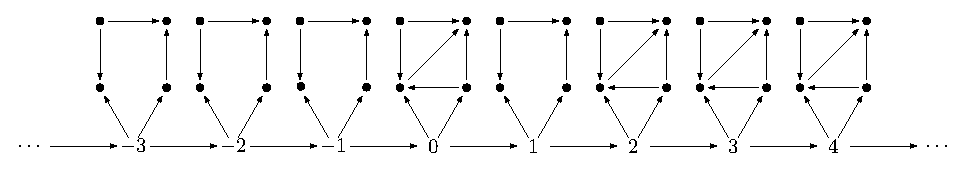
\includegraphics[height=.8in]{fig/5-line.eps}
    \caption{The 5-line.}
    \Description{5-line.}
    \label{fig:5-line}
\end{figure}
% 
\begin{example}
    Consider the graph in Figure~\ref{fig:5-line}.
    Bauslaugh~\cite{bauslaugh1994homomorphisms} proved an 
    endomorphism of this graph must either be the identity; 
    or it map vertex $i$ to vertex $i+k$ where $k \geq 2$,
    where the endomorphism image is like the graph but with 
    no edges inside the pentagon above vertex $0$.
    In this latter case, the image is not isomorphic to 
    the original graph, so it is not a core.
    Yet, the only endomorphism that is a retraction is
    the identity, so it satisfies property R.
\end{example}

\rw{Can we prove our definition of core is weaker than 
$I,S,N$ but stronger than $R$? I.e., 
$I \vee S \vee N \implies \text{core} \implies R$?
Or are they incomparable?}

\subsection{Extending Core Chase to the Infinite Case}
There have been attempts to extend the core chase 
 to the infinite case.
Carral et al.~\cite{DBLP:conf/icdt/CarralK0OR18} define 
 the core in the same way as Bodirsky~\cite{DBLP:journals/lmcs/Bodirsky07}.
Baget et al.~\cite{DBLP:conf/pods/BagetMR23} do not define 
 a core for infinite structures, but study the behavior 
 of the core chase when it does not terminate.

\rw{Can we prove the core chase converges to the infinite core?}

\bibliographystyle{ACM-Reference-Format}
\bibliography{references}

\end{document}